%% Overleaf			
%% Software Manual and Technical Document Template	
%% 									
%% This provides an example of a software manual created in Overleaf.

\documentclass{ol-softwaremanual}

% Packages used in this example
\usepackage{graphicx}  % for including images
\usepackage{microtype} % for typographical enhancements
\usepackage{float}
\usepackage{amsmath}   % for equations and mathematics
\usepackage[a4paper,top=4.2cm,bottom=4.2cm,left=3.5cm,right=3.5cm]{geometry} % for setting page size and
\usepackage{subcaption}
\usepackage[export]{adjustbox}
\usepackage{wrapfig}
\usepackage[spanish]{babel}
\usepackage{array}
\usepackage{etoolbox}
\usepackage{tabularray}
\usepackage{hyperref}  % for hyperlinks

\hypersetup{
    colorlinks=true,
    linkcolor=blue,
    filecolor=magenta,      
    urlcolor=cyan,
    pdftitle={Overleaf Example},
    pdfpagemode=FullScreen,
    }

% Custom macros used in this example document
\newcommand{\doclink}[2]{\href{#1}{#2}\footnote{\url{#1}}}
\newcommand{\cs}[1]{\texttt{\textbackslash #1}}

\begin{document}

\begin{figure}[b]
\centering

\includegraphics[width=0.4\textwidth]{Main/logo-impa.png}
\end{figure}


% Frontmatter data; appears on title page
\softwarelogo{
\includegraphics[width=9cm]{Main/SolarLink logo.png}}
\title{Solar Link \\ Propuesta ambiental de futuro sostenible}
\author{Cenyko, Ivan Ezequiel \\ Dias, Lara Paloma \\ Inza Fior, Mateo \\ Palmieri Hise, Agustín \\ Testa, Maximiliano Nicolas}
\date{\textit{2023}}

\maketitle
\tableofcontents
\newpage

\section{Preámbulo}

\subsection{¿Quiénes somos?}


\begin{table}[!hbt]
\begin{tblr}{c c}
    \SetCell[r=10]{} 
\includegraphics[width=0.35\textwidth]{preambulo/Imagen de WhatsApp 2023-10-14 a las 18.27.44_028dad0b.jpg} 
    & \SetCell[r=1]{l} Ivan Ezequiel Cenyko
    &  \\ 
    &  \\
    & \SetCell[r=1]{l}DNI: 46.028.174
    & \\ 
    &  \\
    & \SetCell[r=1]{l}Mail: ivancenyko@gmail.com  
    &  \\
    &  \\
    & \SetCell[r=1]{l}\href{https://www.linkedin.com/in/ivan-cenyko/}{Linkedin: www.linkedin.com/in/ivan-cenyko/}  
    &  \\
    &  \\
        & \SetCell[r=1]{} Programación en microPython y desarrollo web Back-End
    &  \\ 
    &  \\
\end{tblr}
\label{tab:multicol}
\end{table}

\begin{table}[!hbt]
\begin{tblr}{c c}
    \SetCell[r=10]{} 
\includegraphics[width=0.35\textwidth]{preambulo/Imagen de WhatsApp 2023-10-14 a las 18.27.45_0fd46106.jpg} 

    & \SetCell[r=1]{l} Lara Paloma Dias
    &  \\ 
    &  \\
    & \SetCell[r=1]{l}DNI: 46200006
    & \\ 
    &  \\
    & \SetCell[r=1]{l}Mail: palomadias308@gmail.com
    &  \\
    &  \\
    & \SetCell[r=1]{l}\href{https://www.linkedin.com/in/lara-paloma-dias-598bb9288/}{Linkedin: www.linkedin.com/in/lara-paloma-dias-598bb9288/}  
    &  \\
    &  \\
    & \SetCell[r=1]{l}Desarrollo web Front-End 
    &  \\
    &  \\
\end{tblr}
\label{tab:multicol}
\end{table}

\begin{table}[!hbt]
\begin{tblr}{c c}
    \SetCell[r=10]{} 
\includegraphics[width=0.35\textwidth]{preambulo/Imagen de WhatsApp 2023-10-14 a las 18.27.45_22ea3b81.jpg} 
    & \SetCell[r=1]{l} Mateo Inza Fior
    &  \\ 
    &  \\
    & \SetCell[r=1]{l}DNI: 46.579.589
    & \\ 
    &  \\
    & \SetCell[r=1]{l}Mail: mateoinzafior@gmail.com
    &  \\
    &  \\
    & \SetCell[r=1]{l}\href{https://www.linkedin.com/in/mateoinzafior/}{Linkedin: www.linkedin.com/in/mateoinzafior/}  
    &  \\
    &  \\
    & \SetCell[r=1]{l}Desarrollo web Front-End y programación en microPython
    &  \\
    &  \\
\end{tblr}
\label{tab:multicol}
\end{table}

\begin{table}[!hbt]
\begin{tblr}{c c}
    \SetCell[r=10]{} 
\includegraphics[width=0.35\textwidth]{preambulo/Imagen de WhatsApp 2023-10-14 a las 18.27.46_242e2534.jpg} 
    & \SetCell[r=1]{l} Agustin Palmieri Hise
    &  \\ 
    &  \\
    & \SetCell[r=1]{l}DNI: 46.364.013
    & \\ 
    &  \\
    & \SetCell[r=1]{l}Mail: aguspalmierihise@gmail.com
    &  \\
    &  \\
    & \SetCell[r=1]{l}\href{https://www.linkedin.com/in/agustin-palmieri-hise/}{Linkedin: www.linkedin.com/in/agustin-palmieri-hise/}  
    &  \\
    &  \\
        & \SetCell[r=1]{l} Diseño y confección eléctrico y electrónico íntegro
    &  \\ 
    &  \\
\end{tblr}
\label{tab:multicol}
\end{table}

\begin{table}[!hbt]
\begin{tblr}{c c}
    \SetCell[r=10]{} 
\includegraphics[width=0.35\textwidth]{preambulo/Imagen de WhatsApp 2023-10-14 a las 18.40.11_fa2abbcb.jpg} 
    & \SetCell[r=1]{l} Maximiliano Nicolas Testa
    &  \\ 
    &  \\
    & \SetCell[r=1]{l}DNI: 46.187.213
    & \\ 
    &  \\
    & \SetCell[r=1]{l}Mail: maxitesta2012@gmail.com  
    &  \\
    &  \\
    & \SetCell[r=1]{l}\href{https://www.linkedin.com/in/maximiliano-testa/}{Linkedin: www.linkedin.com/in/maximiliano-testa/}  
    &  \\
    &  \\
        & \SetCell[r=1]{l} Programación en C y desarrollo Front-End de la Web-app
    &  \\ 
    &  \\
\end{tblr}
\label{tab:multicol}
\end{table}

\begin{figure}[H]
    \centering
    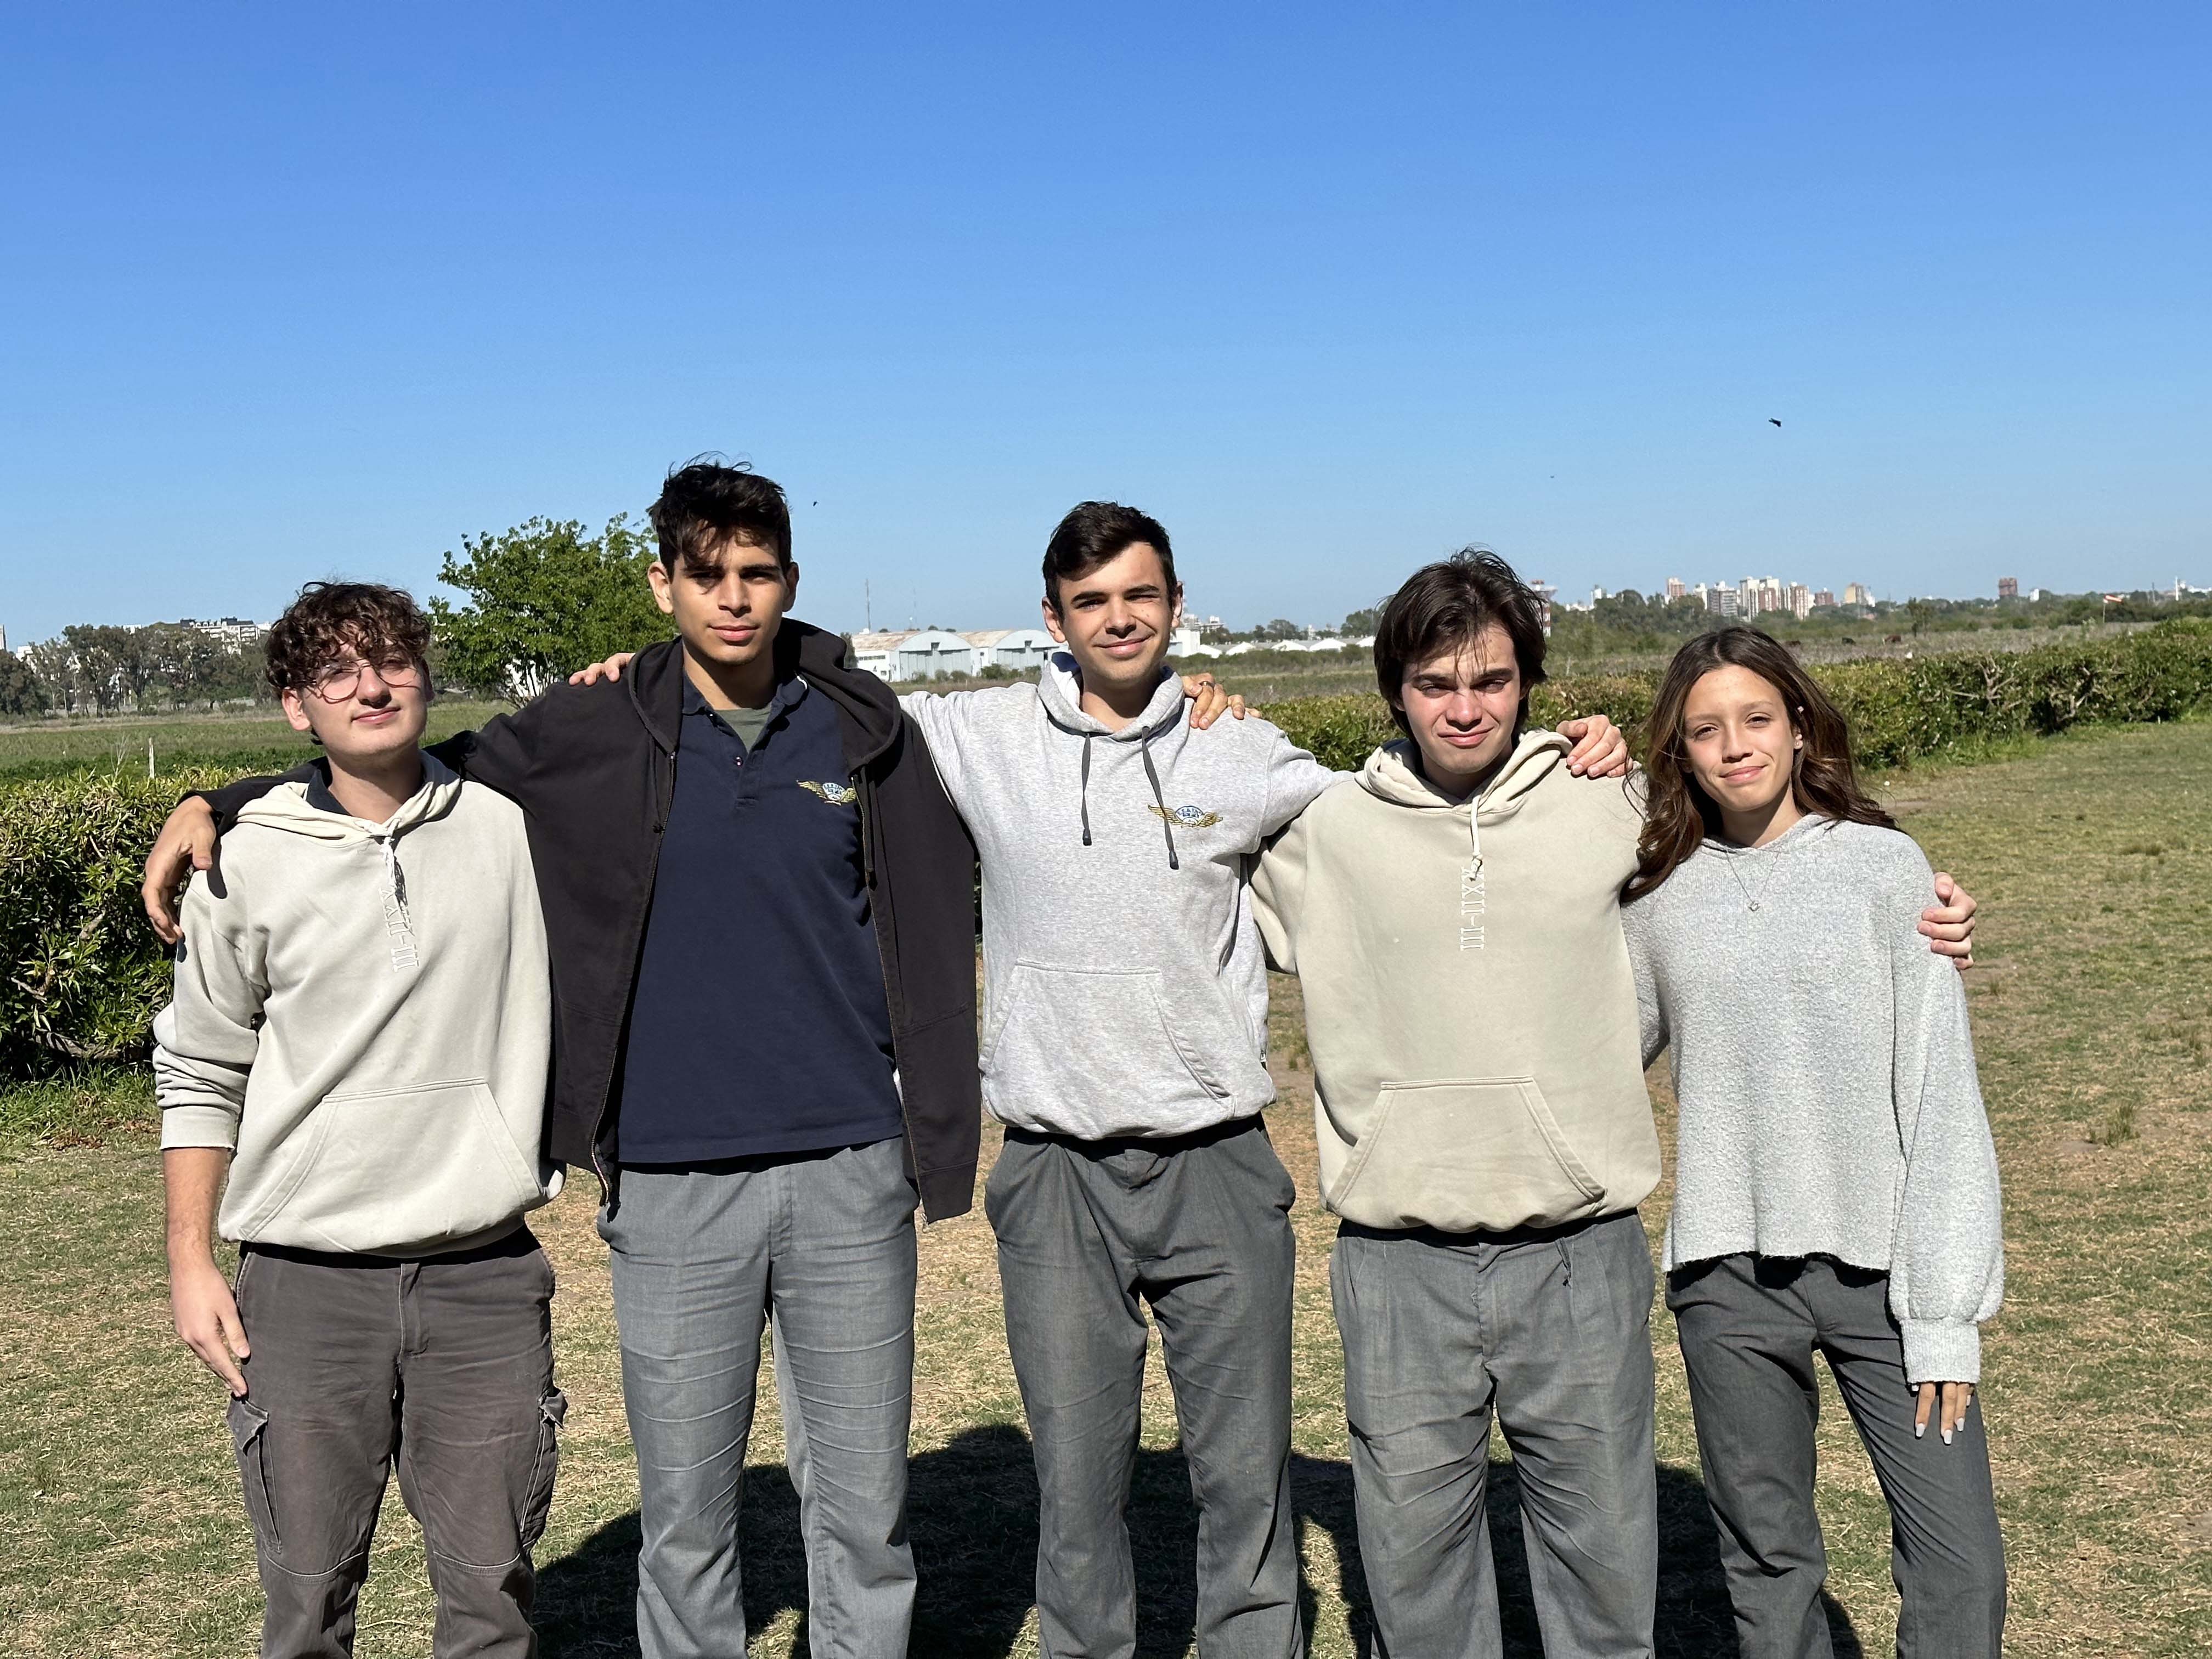
\includegraphics[width=0.85\linewidth]{preambulo/IMG_9428.jpg}
    \caption{Equipo Solar Link}
    \label{fig:equipo solar}
\end{figure}

\begin{figure}[H]
    \centering
    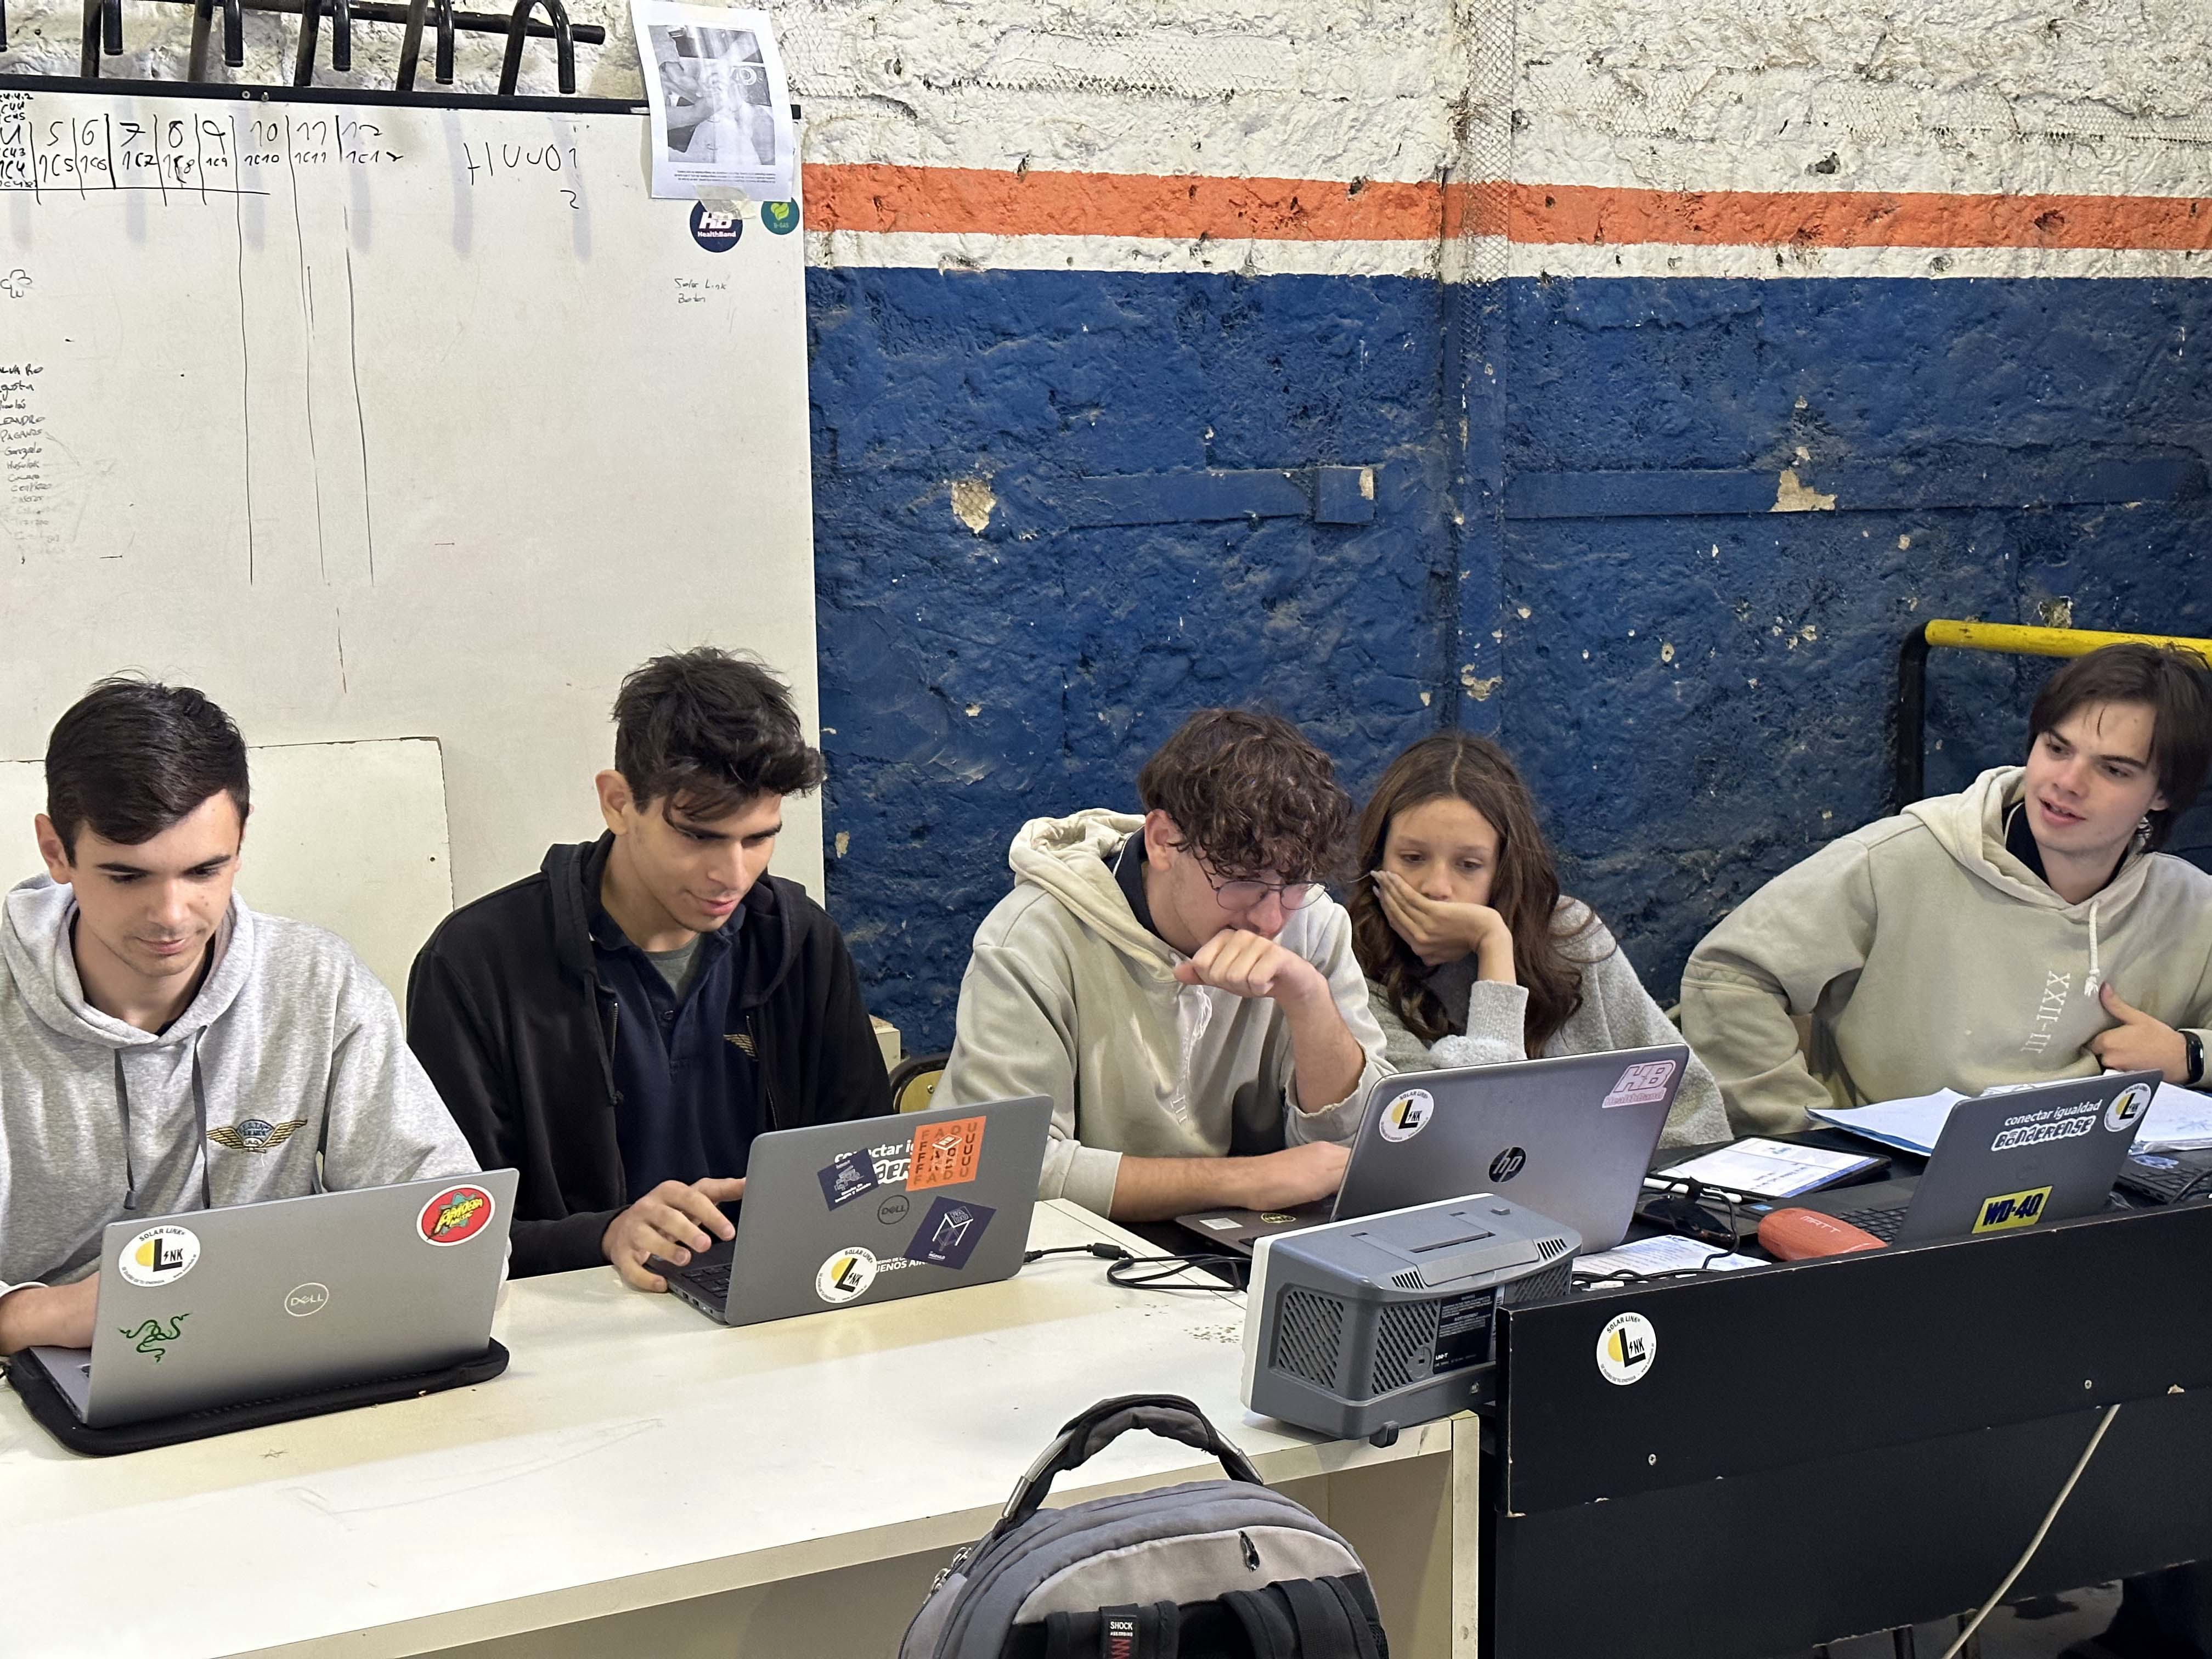
\includegraphics[width=0.85\linewidth]{preambulo/IMG_9439.jpg}
    \caption{Equipo Solar Link trabajando}
    \label{fig:equipo solar laburando}
\end{figure}

\clearpage

\subsection{Contacto}
Podes encontrar a Solar Link en:

\begin{itemize}
\item Mail: info@solarlink.ar
\item Pagina Web: \href{https://www.solarlink.ar}{www.solarlink.ar}
\item Instagram: \href{https://www.instagram.com/solarlink.ar/}{www.instagram.com/solarlink.ar/}
\item Github: \href{https://github.com/solarlink-ar/solarlink}{github.com/solarlink-ar/solarlink}
\item Trello: \href{https://trello.com/w/2023_721c_solarlink}{trello.com/w/2023\_721c\_solarlink}
\end{itemize}

\subsection{Docentes a cargo}

\begin{itemize}
\item Sergio Medina \\ Nos fue de ayuda a la hora de organizar y presentar nuestro proyecto.
\item Fabrizio Carlassara \\ Nos guió en el desarrollo de todo el software del proyecto. 
\item Diego Palmieri \\ Nos prestó las herramientas y los medios necesarios a fin de confeccionar el proyecto.
\end{itemize}

\subsection{Información adicional}

\subsubsection{Tiempo invertido}

\begin{itemize}
\item Fecha de inicio: 20 de noviembre de 2022.
\item Duración: 32 semanas de trabajo.
\item Esfuerzo del proyecto individual: 8 horas de trabajo semanales de cada integrante.
\item Esfuerzo total del proyecto: 1280 horas de trabajo.
\end{itemize}

\subsubsection{Programas utilizados}

\begin{itemize}
\item Visual Studio Code: Fue utilizado como editor de código en diferentes lenguajes.
\item Thonny: Fue utilizado como editor de código para el mirocontroladoor ESP32.
\item KiCad: Fue utilizado para el diseño de todas las PCBs.
\item AutoCad: Fue utilizado para el diseño 3D de las carcasas de las PCBs.
\item Git: Fue utilizado para manejar el código del proyecto entre el grupo.
\item DB Browser: Fue utilizado para leer la base de datos y probar su interacción con lo que programamos.
\item Photoshop: Fue utilizado para el diseño de diferentes imagenes descriptivas del proyecto.
\item Overleaf: Fue utilizado para la realización de la carpeta técnica, de campo y de usuario en LaTex.
\end{itemize}

\subsubsection{Lenguajes de programación y frameworks utilizados}

\begin{itemize}
\item Python: Lógica de página web.
\item MicroPython: Programación del microcontrolador ESP32.
\item C: Programación del microcontrolador Raspberry Pi Pico.
\item Django: Back-end de página web.
\item Microdot: Web de configuración de la ESP32.
\item HTML, CSS: Front-end de la página web.
\item javascript: Front-end de la página web.
\item Terminal de Linux: Manejo de hosting de la web y propósito general.
\item LaTex: Confección de PDFs para carpeta técnica, de campo, y de usuario.
\end{itemize}

\subsection{Agradecimientos}
Este proyecto no hubiera sido posible sin la colaboración de los docentes anteriormente mencionados, la Asociación Cooperadora IMPA y las empresas Eléctrica Bernal, \href{www.bateriasroverano.com.ar}{Roverano}, \href{www.exo.com.ar}{Exo} y \href{www.newtonmicroscopios.com}{Newton Microscopios}.


\clearpage

\section{Resumen del proyecto}

Solar Link es un administrador inteligente de energía eléctrica (Smart Grid) único en su tipo, que busca incentivar y maximizar el uso de energías renovables. A través de paneles solares, y con un sistema inteligente, alimentar todo el consumo hogareño posible con energía solar, “switcheando” las líneas de la casa (ejemplo iluminación, tomacorrientes) entre la línea eléctrica del proveedor (edesur o edenor p/ej) y la alimentación renovable.\\

La aplicación web, vinculada con el tablero del usuario, puede mostrar el consumo hogareño en tiempo real, cuánto se consumió de cada origen y se ahorró en el último tiempo, cuánto significa esto en términos de ahorro de dinero en la factura de luz, a modo de concientización en la importancia del uso de este tipo de energía.\\

En caso de cortes de suministro de luz, Solar Link puede encargarse de lo esencial de la casa que haga falta alimentar, siempre que esté en su margen de funcionamiento. \\

Por último, el proyecto plantea ser modular, versátil y económico, de forma tal que el tablero puede trabajar con cualquier cantidad de paneles o baterías que se le suministren: Solar Link no está limitado sólo a una fuente de energía solar. Aunque el enfoque de nuestro proyecto es aprovechar este tipo de energía, el sistema permite aprovechar también cualquier tipo de fuente: desde una red de proveedor extra, pasando por cosas como un grupo electrógeno, y hasta otras fuentes renovables; biogas, eólica, entre otras. \\


\section{Desarrollo del proyecto}

Nuestra propuesta para solventar algunas desventajas de los sistemas de energía renovable (especialmente la solar) es crear un sistema autónomo e inteligente que, a través de un sistema off-grid, sea capaz de acoplar y desacoplar la casa de la red eléctrica convencional, dependiendo del consumo de la misma.\\

Este sistema debe ser capaz de leer el consumo de las líneas de la casa, y debe conocer la potencia que el sistema solar instalado puede entregar. De esta manera, cuando se detecte que el consumo de la casa puede ser alimentado por el sistema off-grid, dejará de alimentar la casa con el proveedor de energía eléctrica. Mientras que si el consumo supera el límite establecido, volverá a alimentarla. Para realizar esto, se utiliza la técnica “cruce por cero”, para sincronizar el cambio entre líneas, y que no se note este cambio.\\

Puede ocurrir que en una casa estén constantemente heladeras, calefactores, computadoras, y otros electrodomésticos de alto consumo en uso, y que el sistema off-grid nunca pueda ser capaz de alimentar la línea general de la casa. Para esto, proponemos que Solar Link trabaje parcialmente sobre la casa, pudiendo alimentar independientemente la línea de iluminación y la línea de tomas de la casa. Es decir, si se da el caso mencionado anteriormente, la línea de iluminación seguiría siendo alimentada por energía solar, mientras que la línea de tomas la sería alimentada por el proveedor de energía eléctrica.\\

En caso de un corte de suministro de luz,el sistema Solar Link seguiría funcionando, alimentando a la mayor parte de la casa posible.

Un aspecto clave del proyecto es la accesibilidad e interacción con el usuario. Solar Link incluye una aplicación vinculada con sensores distribuidos en la red eléctrica de la casa. El usuario podrá así tener una noción más concreta de cuáles son los principales consumos del hogar, y le brinda la información necesaria a Solar Link para alternar el uso de energía off-grid y energía de red en cada línea modular.\\

Además, para optimizar la carga del sistema solar, desarrollamos un cargador MPPT de 3 etapas que no solo le da la mejor carga posible a las baterías del sistema, sino que también monitorea el estado de carga de las mismas, y se lo comunica al módulo Solar Link para tenerlo en cuenta a la hora de la conmutación entre lineas, y a la hora de entregarle la mayor cantidad de información posible sobre el sistema al usuario.\\

\clearpage

\section{Impacto ambiental}

\subsection{El aspecto de energías no renovables}

Las principales fuentes de energía con las que cuenta hoy el mundo, petróleo, gas natural y carbón mineral, son de carácter no renovable o convencional; es decir que a medida que se van consumiendo disminuyen sus reservas sin posible reposición, salvo que se descubran nuevos yacimientos.\\

Este sector de energías convencionales sigue teniendo un papel protagónico en la matriz energética mundial, producto de un mercado con muchos años de desarrollo tecnológico, con un gran capital hundido en infraestructura, costos competitivos y con porcentajes de rendimiento y de potencia firme superiores a las renovables. Sin embargo, el consumo de combustibles de origen fósil tiene un efecto muy negativo para el medio ambiente, ya que el dióxido de carbono que se produce por su combustión es el principal constituyente de lo que se conoce como gases de efecto invernadero, principales responsables del calentamiento global.\\

Las consecuencias de este efecto son, por ejemplo, el aumento de las temperaturas, los picos de temperaturas extremos, que han venido manifestándose en los últimos años. Es por ello, que las emisiones globales de carbono continúan aumentando, lo que indica la necesidad de un conjunto integral de medidas políticas para lograr la reducción sustancial de las emisiones de carbono.\\

\begin{figure}[H]
    \centering
    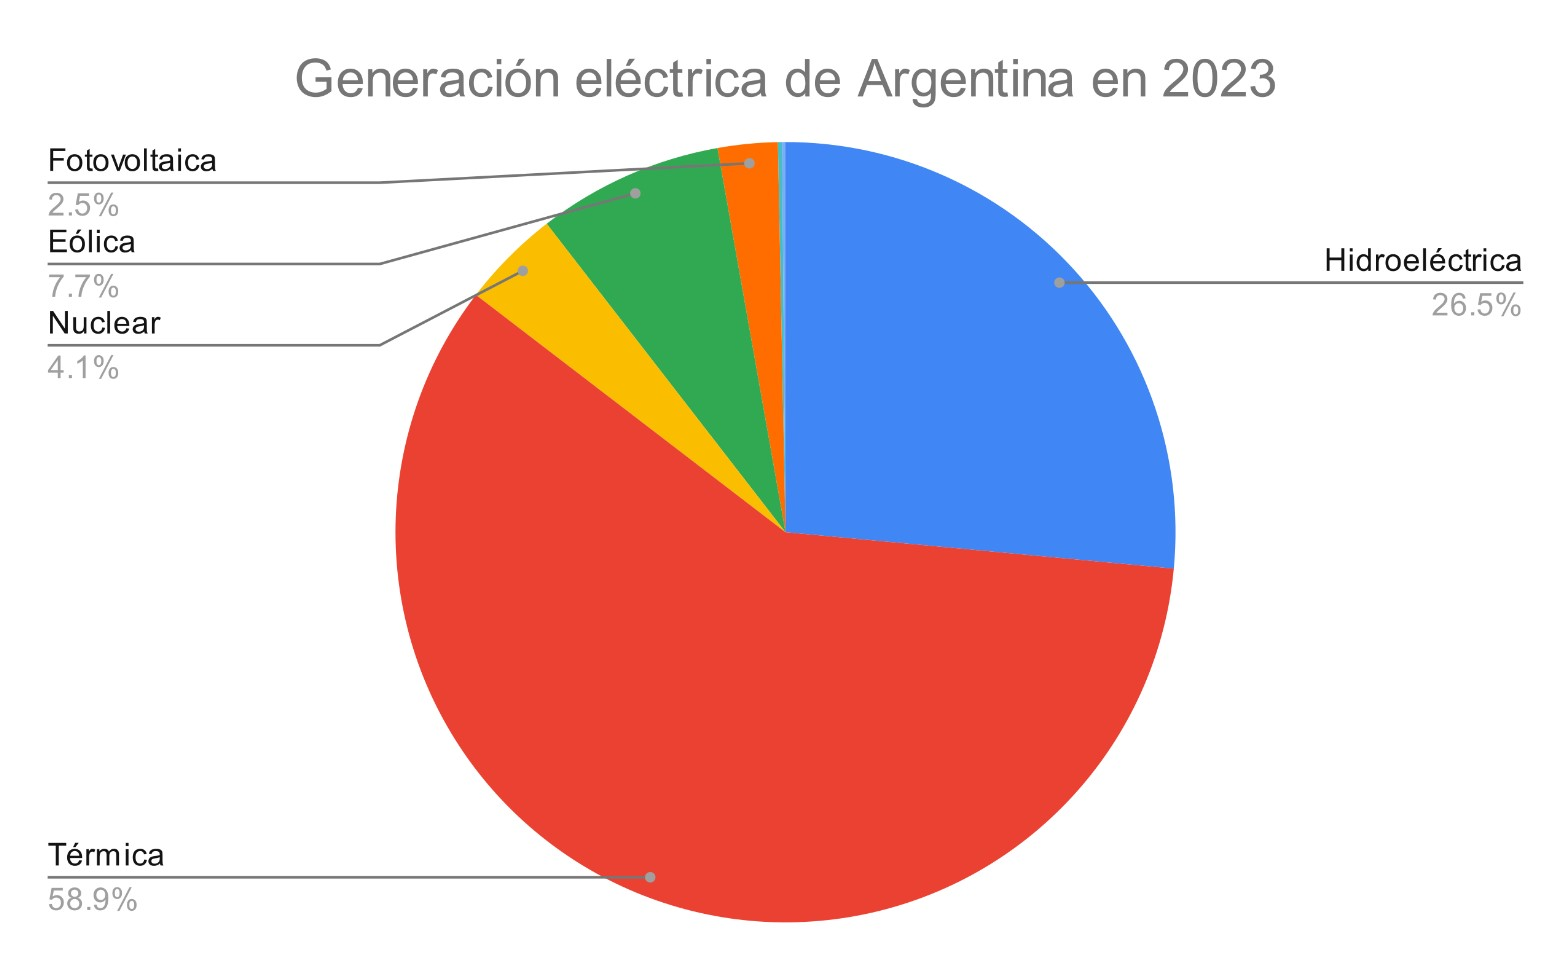
\includegraphics[width=0.85\linewidth]{ambiente/Screenshot_20.jpg}
    \caption{Matriz de generación energética en Argentina}
    \label{fig:matriz-energias}
\end{figure}

En Argentina, casi el 60\% de la energía producida y distribuida en el país son de carácter no renovable. La visión de Solar Link es aportar a que ésta brecha vaya disminuyendo hasta su exterminacion, volviendo a las energias renovables cabecillas en la generacion de energia. \\

\subsection{Uso de baterías en la actualidad}
En la actualidad, las baterías de litio están tomando cada vez mas protagonismo en el mercado. Estas, luego de su uso, se vuelven obsoletas y generan desechos que no son reciclables, sin contar que su extracción es altamente nociva y genera residuos contaminantes. \\

La solución que nosotros proponemos es impulsar el uso de baterías de plomo ácido, que no solo son reciclables hasta en un 80\%, sino que tienen una expectativa de vida mayor. Esto sumado al cargador MPPT de Solar Link, que maximiza el potencial recibido de una fuente de energía renovable y la vida útil de las baterías, creemos que es una solución tanto viable como económica. \\

\subsection{El aspecto de la energía solar}
El sol es el mayor suministro de energía que dispone la humanidad disponible de forma ilimitada
y que puede ser aprovechada en cualquier parte del mundo. Existen dos maneras principales de capturar esta energía solar: la fotovoltaica y la térmica, ambas comparten la virtud que pueden ser producidas y consumidas en cualquier lugar, tanto en áreas remotas o grandes ciudades.\\

En las economías emergentes, como la Argentina, donde existe déficit de infraestructura en
generación, transporte y distribución, esta energía permite soluciones de generación a los
individuos o poblaciones aisladas.

\begin{figure}[H]
\centering
\begin{subfigure}{0.4\textwidth}
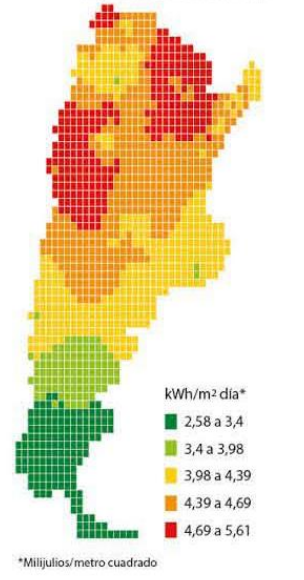
\includegraphics[width=1\linewidth]{ambiente/Screenshot_1.png} 
\caption{Zonas del pais con mayor \\promedio de intensidad de \\radiación solar}
\end{subfigure}
\begin{subfigure}{0.4\textwidth}
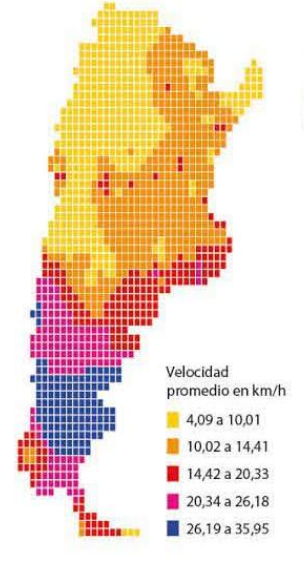
\includegraphics[width=1\linewidth]{ambiente/Screenshot_2.png}
\caption{Zonas del pais con mayor \\promedio de intensidad de \\los vientos}
\label{fig:subim2}
\end{subfigure}
\label{fig:image2}
\end{figure}

Nótese que justamente las provincias con más potencial solar (inclusive eólico) son aquellas donde el consumo de energía eléctrica es mucho más caro en comparación con el gran Bs As y otros centros urbanos, principalmente por los altos costos de distribución de energía. Acá es donde Solar Link tendría su mayor aprovechamiento.\\

Considerando la estadística mostrada, un metro cuadrado de panel solar (en bs as) podría generar 4 kW/h por día. Suponiendo que el panel está en uso 12hs por día, se generan 330 W/h por metro cuadrado de panel. 
En realidad, los paneles son menos eficientes que esto, por tanto para recibir esos 330W/h los paneles son más grandes que 1 metro cuadrado. \\
Sabiendo esto, usaremos como ejemplo un panel solar de 380 W/h y 1.75 metros cuadrados. Por tanto durante, en promedio, 12 hs, se recibirán 380 W/h en el panel. Esta generación de energía implica que por día se producen 4.56 kW/h.\\

En promedio, por mes, una casa de núcleo familiar consume 600 kW/h, o sea 20 kW/h por día. Si hacemos números, nos da que el sistema sería capaz de alimentar con energía solar el 25\% de esa carga (en promedio), ya que de los 600 kW/h por mes, 140 pudieron generarse con el sistema para cargar las baterías y que estas después alimenten las líneas competentes. \\

Hoy en dia el desarrollo de la tecnologia relacionado con la energía solar crece exponencialmente, haciendo mas barato y accesible estos sistemas. A su vez, en argentina disminuye el subsidio destinado a la distribución eléctrica, cerrando lentamente la brecha monetaria entre pagar la luz y recurrir a energias renovables. \\

Teniendo en cuenta todo lo dicho anteriormente, el uso de energias renovables no solo se esta volviendo plausible, sino que tambien se esta volviendo rentable y accesible. Nuestro objetivo con Solar Link es volver esta esperanza en una realidad. \\

\section{Beneficios sociales}

\subsection{Beneficio económico}

Solar Link propone el uso de un sistema solar off-grid de baja potencia, el cual es la alternativa mas económica que se consigue de energía solar. Este sistema consta de panel/es solar/es, batería/s, nuestro cargador MPPT de 3 etapas y un inverter. \\

El sistema que recomendamos instalar en un hogar promedio en Argentina, se compone de dos paneles solares de 380W, un inverter de 2000W, dos baterías de ciclo profundo de 110Ah, el cargador MPPT de 3 etapas de Solar Link, y el módulo Solar Link, con un costo total aproximado de esto ARS \$1.600.000 (USD \$1.600).\\

Mientras tanto, un sistema comparable on-grid, puede salir ARS \$5.000.000 (USD \$5.000). Esto depende del servicio que se contrate y de la empresa que lo realice.\\

No está de más mencionar que al uno producir la energía  que consume, se disminuye el consumo de energía de terceros, el del proveedor eléctrico. Esto quiere decir, que todos los meses se verá reducido el precio que hay que pagar por el suministro de energía eléctrico.\\

El ahorro en este caso no es lineal. Si uno termina consumiendo a fin de mes la mitad de energía que consumiría normalmente, por como funciona el sistema de cobros de las empresas distribuidoras en Argentina, no pagaría la mitad, sino que bastante menos.\\

Esto ocurre porque las empresas establecen un precio para cada KW/h dependiendo de la escala en donde se consuma. Por ejemplo, entre 0KW/h y 200KW/h tiene un precio asignado, entre 200KW/h y 400KW/h otro mayor, y si se exceden esos 400KW/h otro inclusive mayor (estas escalas dependen de la empresa a cargo del suministro eléctrico).\\

Osea, digamos, que cada KW/h entre 0KW/h y 200KW/h valga 1, entre 200KW/h y 400KW/h, 1,5, y si es mayor a 400KW/h, 2. si uno consume 600KW/h, estaría pagando 900, mientras que si uno consume 300KW/h, estaría pagando 350, bastante menos de la mitad. Este ejemplo ilustra como funciona el sistema de cobros de las compañías distribuidoras en Argentina. Las escalas y los valores son a modo de ejemplo. Pueden ser diferentes segun la empresa, la región, y el momento en donde se analice.\\

\subsection{Incentivo y concientización}

A través de nuestra aplicación, el usuario tendrá acceso a toda la información que respecta al consumo eléctrico de su casa. Esto le permite conocer al detalle no solo el consumo total, sino tambien el consumo que generó el sistema solar propio.\\

Esto genera en el usuario un sentido de ganancia y de gasto propio. Saber bien cuanto se esta gastando, porque y cuanto de este gasto se amortiguo ayuda a concientizar sobre el consumo de energia en general. \\

Mas allá del gasto de energía, tener un sistema que, ya sea de manera directa o indirecta, ayuda al medio ambiente, tiene un efecto positivo para la psiquis y para el entorno donde uno vive. Saber que uno esta aportando su grano de arena (siendo el mismo economicamente viable y rentable) genera tranquilidad y un sentido de responsabilidad ciudadana. \\

\subsection{Estado del arte}

Actualmente, en el mercado argentino, existen principalmente tres tipos de instalaciones de energía solar para un hogar. Cada tipo cuenta con sus propias ventajas y desventajas:\\

\begin{table}[H]
\begin{tabular}{|l|l|l|}
\hline
Tipo     & Ventajas                                                                                                                 & Desventajas                                                                                            \\ \hline
On-Grid  & \begin{tabular}[c]{@{}l@{}}Sistema acoplado a la línea doméstica\\ Alimenta casi el 100\% con energía solar\end{tabular} & \begin{tabular}[c]{@{}l@{}}Alto costo\\ Desperdicio de energía\end{tabular}                            \\ \hline
Off-Grid & \begin{tabular}[c]{@{}l@{}}Económico\\ Acumula energía\end{tabular}                                                      & \begin{tabular}[c]{@{}l@{}}Requiere una línea exclusiva \\ para este sistema\end{tabular}              \\ \hline
Híbrido  & \begin{tabular}[c]{@{}l@{}}Sistema acoplado a la línea doméstica\\ Acumula energía\end{tabular}                          & \begin{tabular}[c]{@{}l@{}}Potencia limitada\\ Requiere instalación especial\end{tabular} \\ \hline
\end{tabular}
\end{table}

Los sistemas \textbf{on-grid}, como su nombre lo indica, se instalan directamente en la línea de la casa. Toda la energía que producen los paneles se entregan a la línea general de la casa, sin almacenarse en ningún lado. Si la casa consume mas que lo que generan los paneles, se consume la energía correspondiente a este exceso del proveedor eléctrico, y si consume menos, la energía generada por demás se entrega a la red eléctrica del proveedor. \\

Para este tipo de sistemas es necesaria la instalación de un medidor bidireccional, que mide tanto el consumo de la casa como lo que devuelve por el exceso en la producción. Si bien este medidor descuenta lo que uno devuelve a la red eléctrica, lo que uno consume es mas caro, no es muy redituable y no su instalación depende del proveedor de energía eléctrica.\\

Los sistemas \textbf{off-grid}, por otra parte, acumulan la energía generada por los paneles solares en baterías, para luego convertirla en los 220Vac que necesita la casa. El problema de esto, es que la energía extraída de las baterías no se puede incorporar directamente a la línea de la casa, por lo que es necesario la utilización de una línea exclusiva para lo que este sistema genere. Esto implica tener que hacer una instalación eléctrica aislada e independiente del resto de la casa, algo impráctico si además se tiene en cuenta que la utilización de esta línea debe ser controlada y depende directamente de la carga de los paneles.\\

Los sistemas \textbf{híbridos} son sistemas solares off-grid que se incorporan a la línea de la casa. Pueden utilizar tanto la energía solar acumulada como la energía del proveedor eléctrico. Para utilizar este tipo de sistema es necesaria una instalación especial, que se tiene que realizar en líneas dedicadas. Además, por como es su principio de funcionamiento, el sistema solar no es expandible, por lo que la potencia instalada en un principio no podrá modificarse.\\

Mientras tanto, \textbf{Solar Link} busca recopilar todas las ventajas de estos 3 tipos de sistemas solares, y dejar en el camino todas las desventajas posibles. Se podría decir que Solar Link es un sistema que acumula y utiliza energía solar, acoplado a la línea de la casa, económico, modular expandible y amigable con el usuario, compartiendo toda la información necesaria sobre el sistema solar instalado y el consumo de la casa.


\section{Conclusiones}

Solar Link aprovecha sus cualidades como gestor inteligente para poder aprovechar la energía solar al máximo. Usualmente, la instalación de una fuente de energía solar por sí sóla no daría abasto para toda la casa (recordemos que en nuestro ejemplo sólo cubría el 30\%), y otros tipos de implementación alternativas a una red inteligente serían rígidas e ineficientes. A través de Solar Link, buscamos que con el control automático de consumo y la separación modular de las redes de la casa logremos maximizar la eficiencia en el consumo, y minimizar los gastos posibles.\\

Nuestro objetivo es introducir al país un sistema capaz de evitar energía cuya generación es, en su mayoría, resultado de fomentar el cambio climático, introduciendo energías renovables y control y concientización del consumo a sus usuarios, en otras palabras un smart grid con energías renovables. Por otro lado, otorga a sus usuarios energía generada por ellos mismos para su hogar, y por lo tanto, no deben pagar por ella. \\

Entre sus beneficios están, el uso de energías renovables, la producción de energía en el propio entorno de uso, que reduciría el consumo en la boleta, una aplicación web que permite ver el consumo y configurarlo, dando control al usuario de su consumo y que sea consciente de este. 

\section{Anexo}

\subsection{Referencias}
\href{https://repositorio.uca.edu.ar/bitstream/123456789/11949/1/Bassani%20Mariano.%20TRABAJO%20FINAL%20DE%20MBA_MB_20210311_v2.pdf}{Trabajo final de Facultad de Ciencias Económicas de la UCA: ¿Es negocio invertir en generación eléctrica solar en Argentina?}\\

\href{https://www.un.org/es/chronicle/article/la-promesa-de-la-energia-solar-estrategia-energetica-para-reducir-las-emisiones-de-carbono-en-el#:~:text=De%20acuerdo%20con%20la%20Federaci%C3%B3n,ahorrar%20600%20kilogramos%20de%20CO2}{Organización de las Naciones Unidas: La promesa de la energía solar: Estrategia energética para reducir las emisiones de carbono en el siglo XXI}\\

\href{https://ri.conicet.gov.ar/handle/11336/182578?show=full}{Estado del arte de la tecnología de celdas solares basadas en semiconductores}\\

\end{document}
